\documentclass[11pt,a4paper]{ctexart}
\usepackage[margin=2.3cm]{geometry}
\usepackage{graphicx}
\usepackage{booktabs}
\usepackage{tabularx}
\usepackage{caption}
\usepackage{float}
\captionsetup{font=small,labelsep=quad}
\setlength{\parindent}{2em}
\linespread{1.35}\selectfont
\graphicspath{{../求解结果/图表/}}

\begin{document}

\begin{center}
{\zihao{2}\heiti 问题四\ 仿真过程与可视化结果}\\[6pt]
{\zihao{4}队伍编号：MCB2600843\quad 题号：B}\\[2pt]
{\zihao{5}2026年10月30日}
\end{center}

\vspace{0.5em}

\section*{一、仿真目标与输入}
问题四要求在给定灾前地形、源区体积和传播参数下，给出过程沿沟演进、口岸到达时间、运程及影响强度。本文使用两套相互独立的计算引擎：一维纵剖面模型用于检验准恒定断面下的自然停止与沿程尺度；D8网络模型用于显式连续性推进，输出首达时间场、历史峰值、终态泥深场和质量收支。两套引擎共用同一公共注入断面和同一口岸代理断面，计时均从注入断面开始。

仿真采用附件7的事件日期DEM，主网格约30.71 m（南北）×27.20 m（东西）。源区体积取链A混合入沟体积$2.635835\times10^6$ m$^3$，以集中有限历时源项注入公共断面。D8网络的路由、屈服门槛和Manning阻力参数见表\ref{tab:params}。

\begin{table}[H]\centering\small
\caption{D8仿真基准参数}\label{tab:params}
\begin{tabular}{@{}l c c l@{}}
\toprule
参数&取值&单位&含义\\
\midrule
$V_{\mathrm{target}}$&2635835.294118&m$^3$&链A混合入沟体积\\
$n$&0.10&s/m$^{1/3}$&等效Manning糙率\\
$\tau_y$&800&Pa&屈服门槛\\
$C_v$&0.45&1&岩相体积分数情景\\
$S_{\min}$&0.02&1&缓坡驱动下限\\
$\tau_{\mathrm{src}}$&1800&s&三角源项历时\\
$h_{\min}$&0.10&m&首次到达分析阈值\\
$C_{\mathrm{CFL}}$&0.2&1&Courant上限\\
$T_{\mathrm{end}}$&21600&s&最长演算时限\\
\bottomrule
\end{tabular}
\end{table}

\section*{二、仿真流程}
仿真按以下步骤执行。
\begin{enumerate}
  \item 对DEM作Priority-Flood填洼，按米制最大下坡选择唯一D8受体，并记录每格面积$a_i$、有效过流宽度$W_i$和源项$q_i^{\mathrm{src}}$。
  \item 在公共注入断面按三角源项注入混合体积。源项在$\tau_{\mathrm{src}}=1800$ s内完成，累计注入量等于$V_{\mathrm{target}}$。
  \item 对每格采用显式有限体积更新：
  \begin{equation}
  \frac{\mathrm dh_i}{\mathrm dt}=
  \frac{\sum_{j\in\mathrm{rec}(i)}Q_j-Q_i}{a_i}+q_i^{\mathrm{src}},
  \qquad
  Q_i=\begin{cases}
  n^{-1}h_i^{5/3}\sqrt{S_{\mathrm{eff},i}}\,W_i,&
  \rho_{\mathrm{df}}gh_iS_{\mathrm{eff},i}\ge\tau_y,\\
  0,&\mbox{其他},
  \end{cases}
  \end{equation}
  其中$S_{\mathrm{eff},i}=\max(S_i,S_{\min})$。
  \item 每步按实际波速计算Courant数，超过上限时缩短步长；同步累计注入、域内、出域和损失体积，形成质量账本。
  \item 输出首达时间场、历史最大泥深与峰速、终态泥深场、质量收支和终止状态。首达定义为$t_{\mathrm{arr},i}=\inf\{t:h_i(t)\ge h_{\min}\}$。
\end{enumerate}

除基准配置外，另对体积、糙率、屈服门槛和源项历时等参数作单因素扰动，形成16个去重D8配置，用于考察结果对参数的情景敏感性；这些配置等权展示，不表示现实发生概率。

\begin{figure}[H]\centering
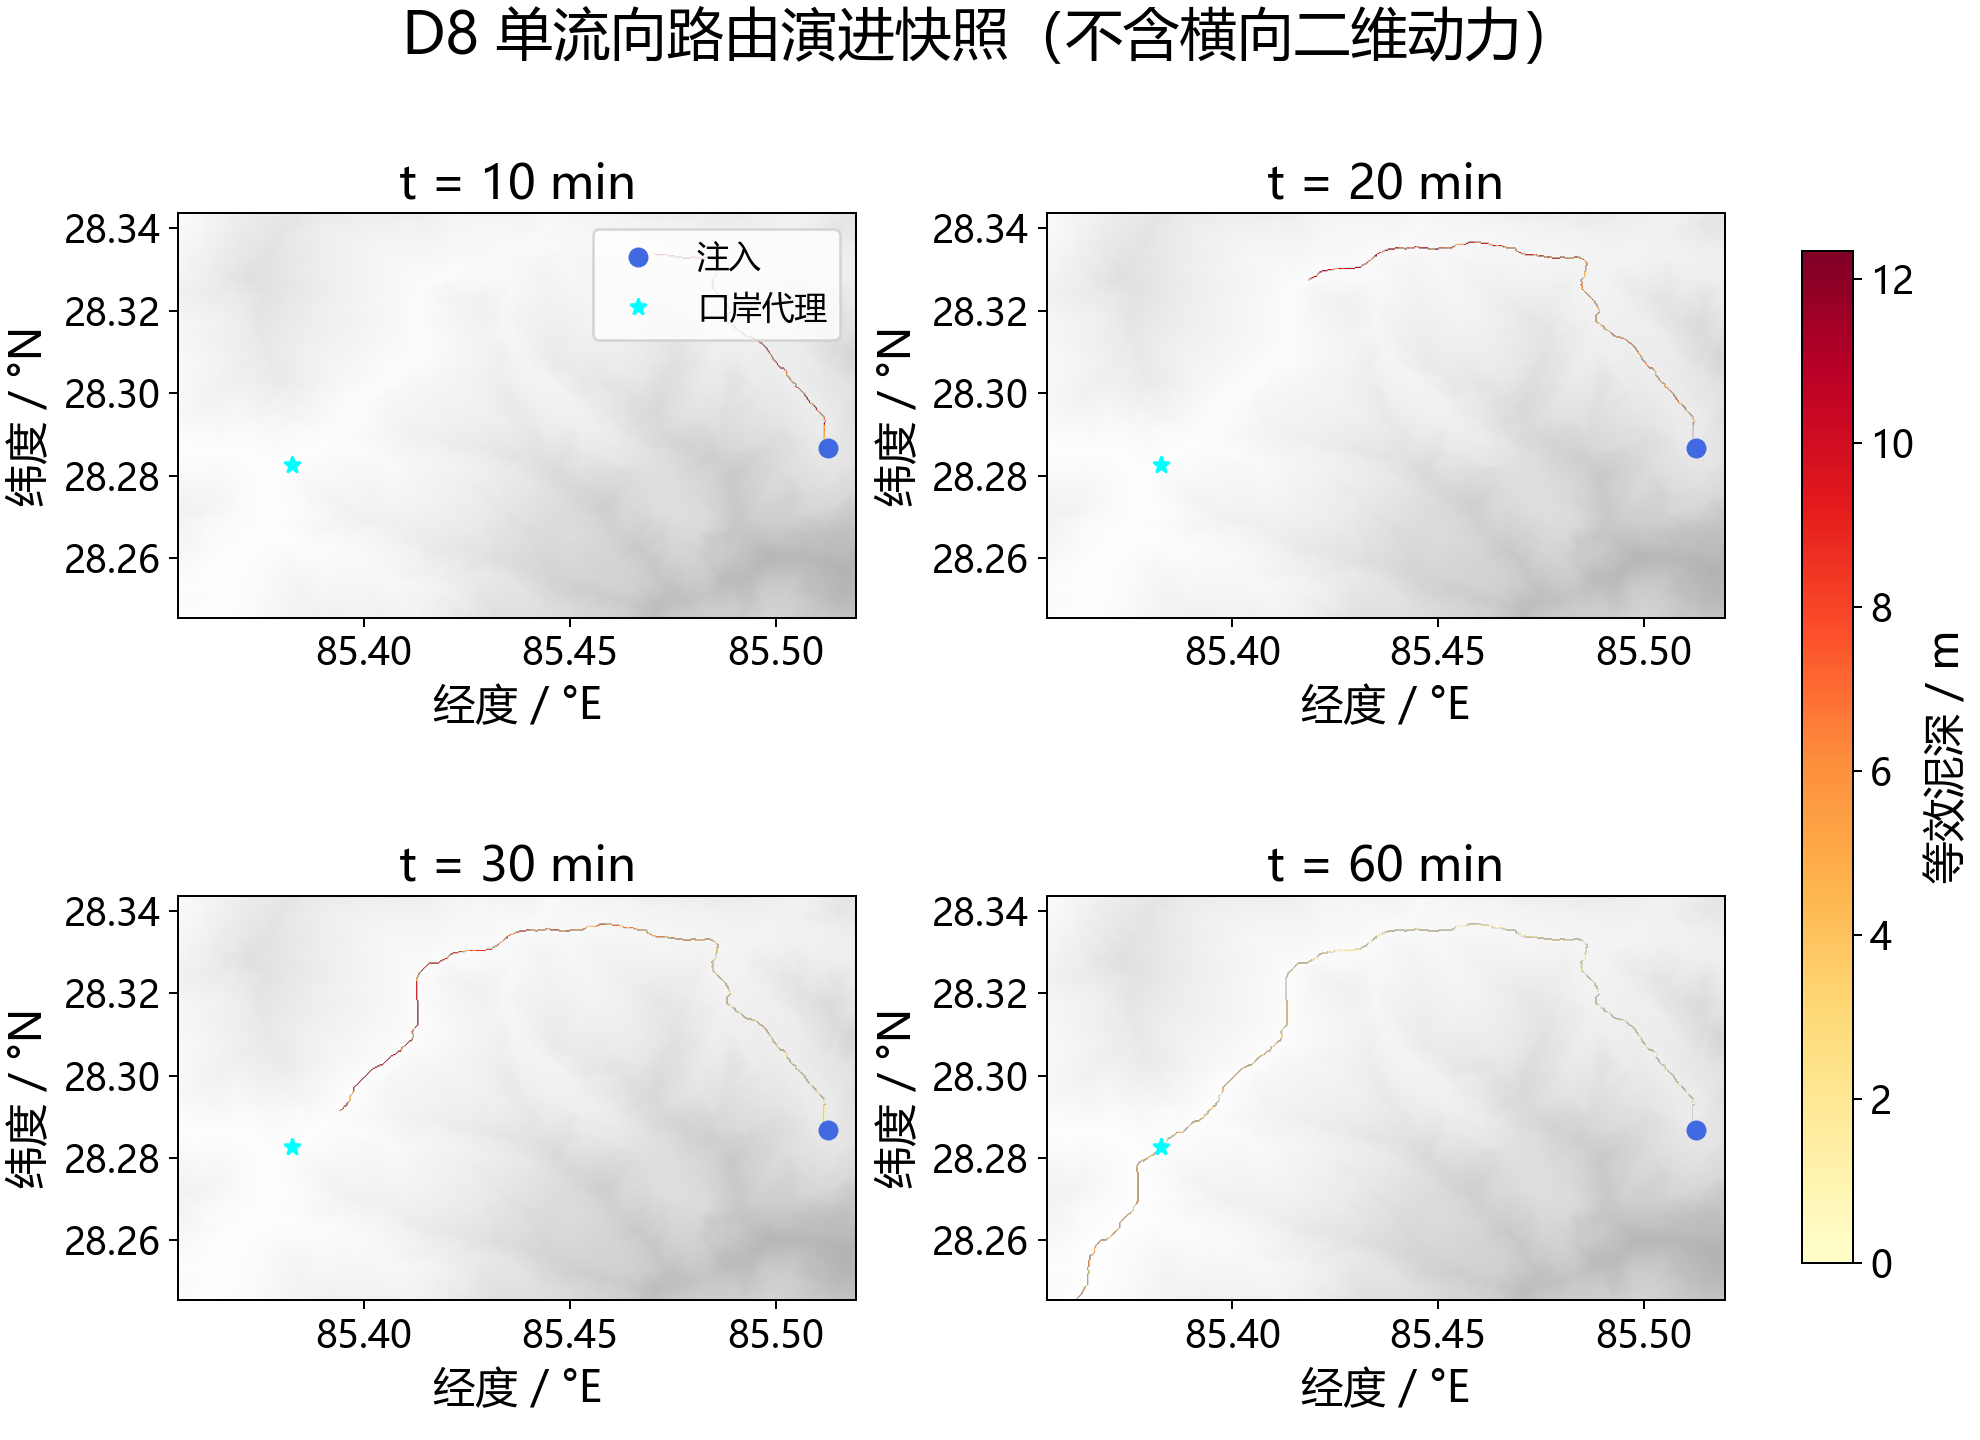
\includegraphics[width=0.96\textwidth]{04b_过程快照.png}
\caption{D8单流向路由演进快照（10、20、30、60 min）}
\label{fig:snapshots}
\end{figure}

\section*{三、可视化仿真结果}
\subsection*{3.1 到达时间与终态泥深}
图\ref{fig:arrival}给出首次达到分析泥深阈值的到达时间场和分析域末端终态泥深。基线口岸代理首达为1965.996174 s，即32.766603 min；16个配置的首达范围为17.5704376--44.7278067 min。全部配置均终止于26045.4946703 m分析域末端的右删失，因此该末端里程是计算范围，不是自然停积边界。

\begin{figure}[H]\centering
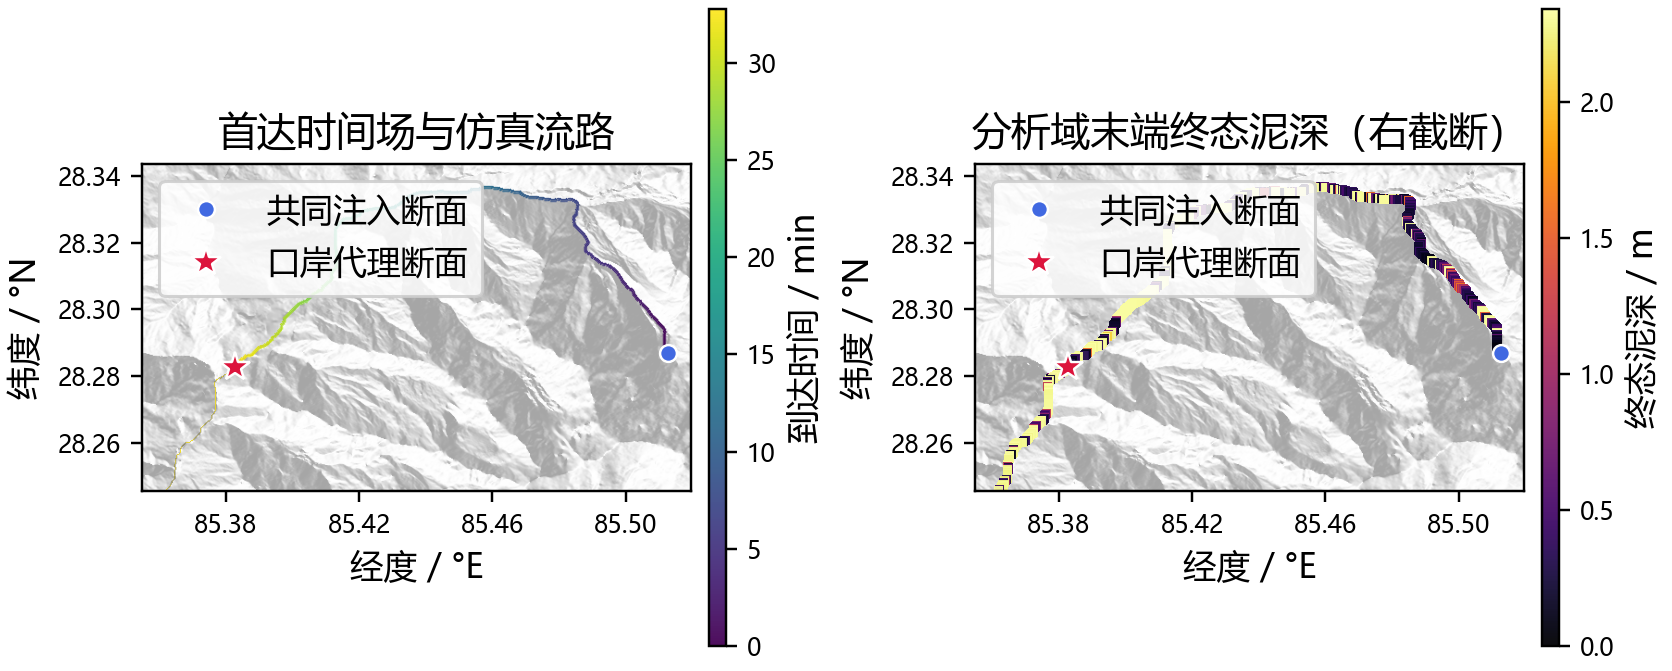
\includegraphics[width=0.96\textwidth]{04b_到达与停积.png}
\caption{首达时间场与终态泥深（分析域末端右删失）}
\label{fig:arrival}
\end{figure}

\begin{figure}[H]\centering
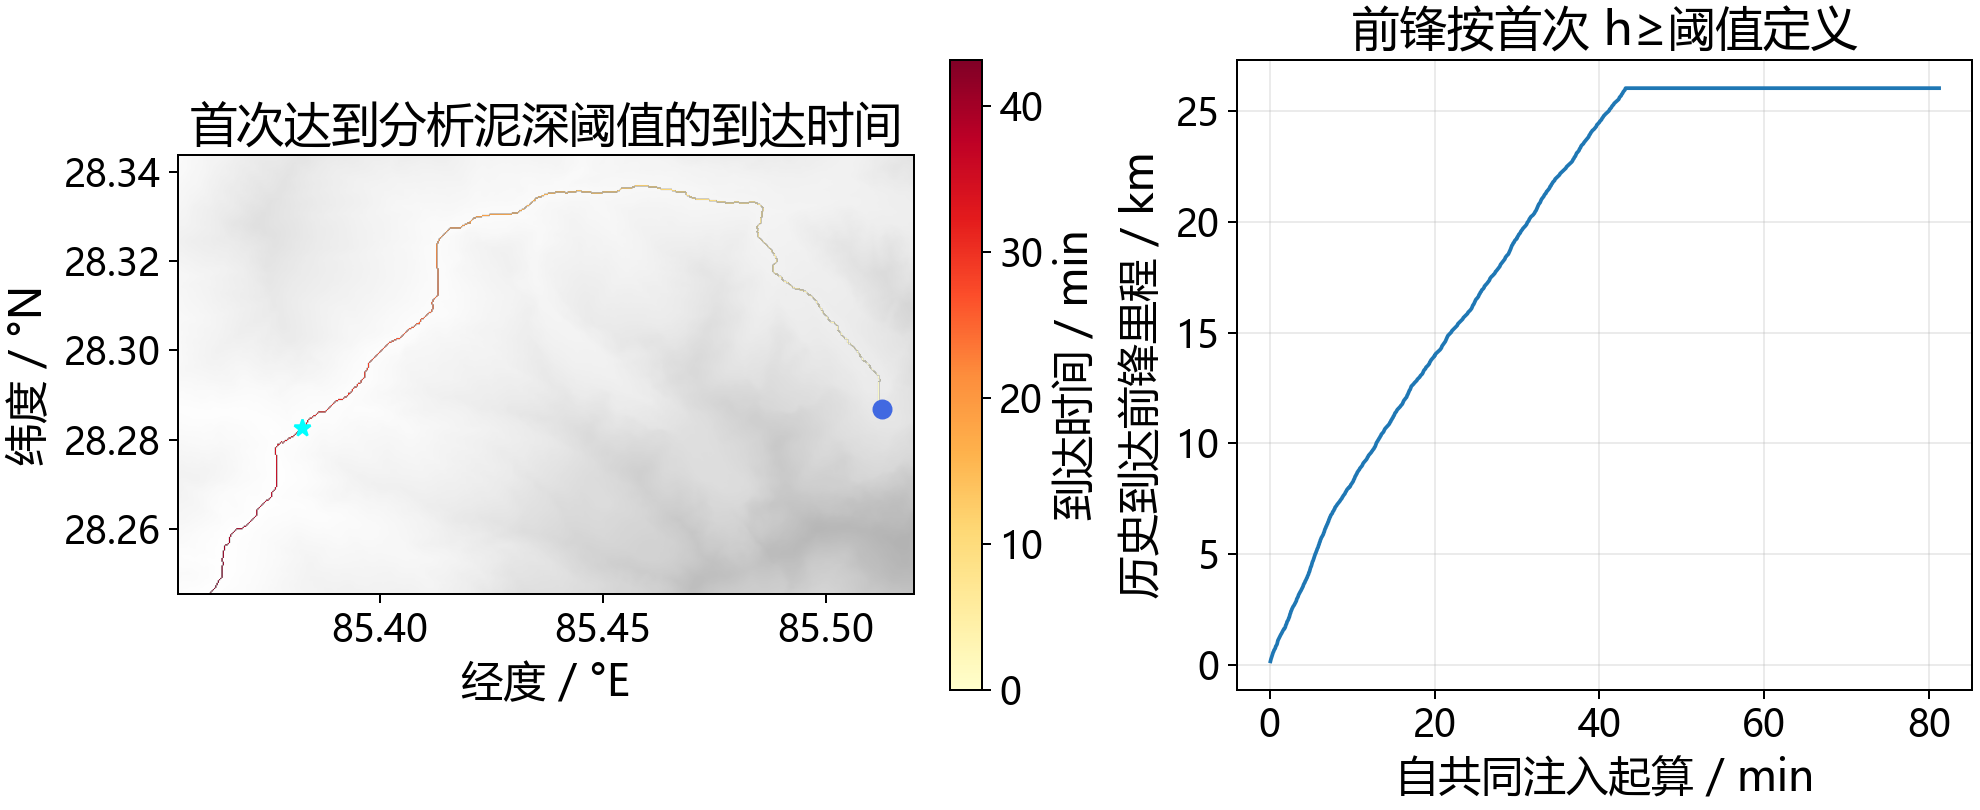
\includegraphics[width=0.96\textwidth]{04b_到达与前锋.png}
\caption{到达时间与前锋沿程距离}
\label{fig:front}
\end{figure}

\subsection*{3.2 峰值、终态与情景差异}
基线口岸历史峰深为10.08530186 m，口岸终态深度为2.298002229 m，全域历史最大深为13.31272084 m，口岸峰值速度为6.601474228 m/s。图\ref{fig:peak}并列历史最大泥深与终态泥深，说明峰值与终态不能互相替代；图\ref{fig:sensitivity}给出16个唯一配置的口岸到达时间。

\begin{figure}[H]\centering
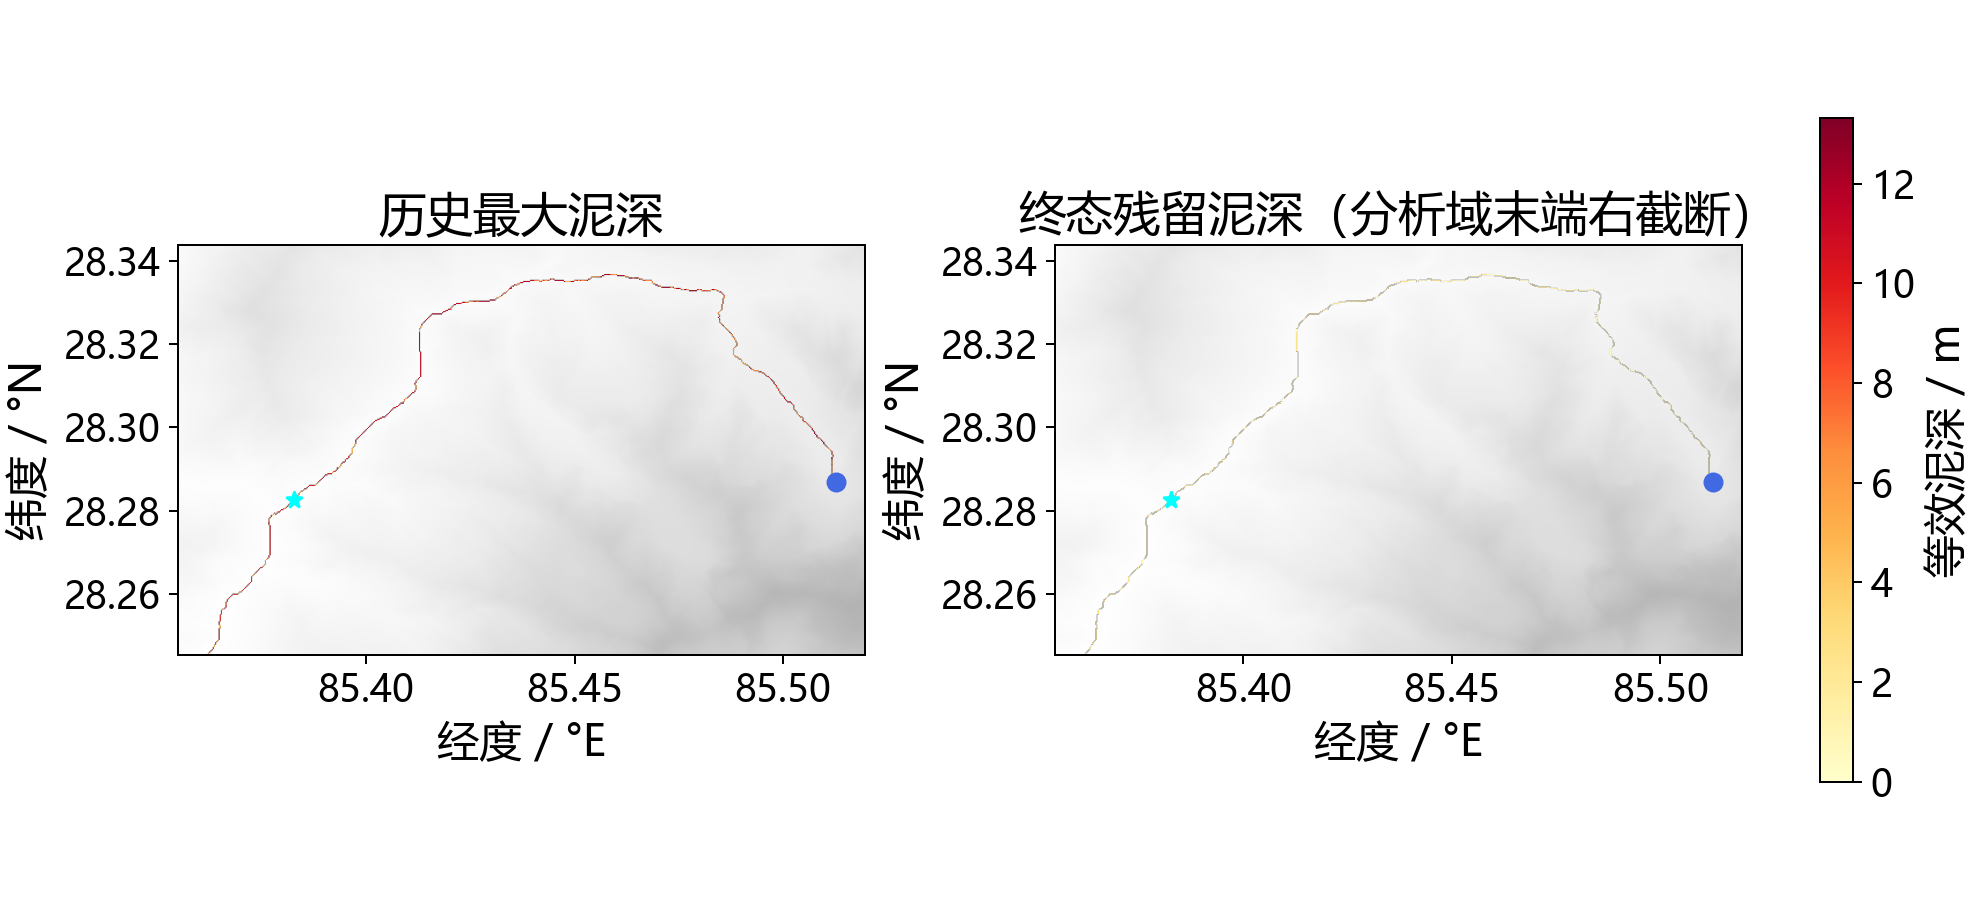
\includegraphics[width=0.96\textwidth]{04b_峰值与终态.png}
\caption{历史最大泥深与终态泥深}
\label{fig:peak}
\end{figure}

\begin{figure}[H]\centering
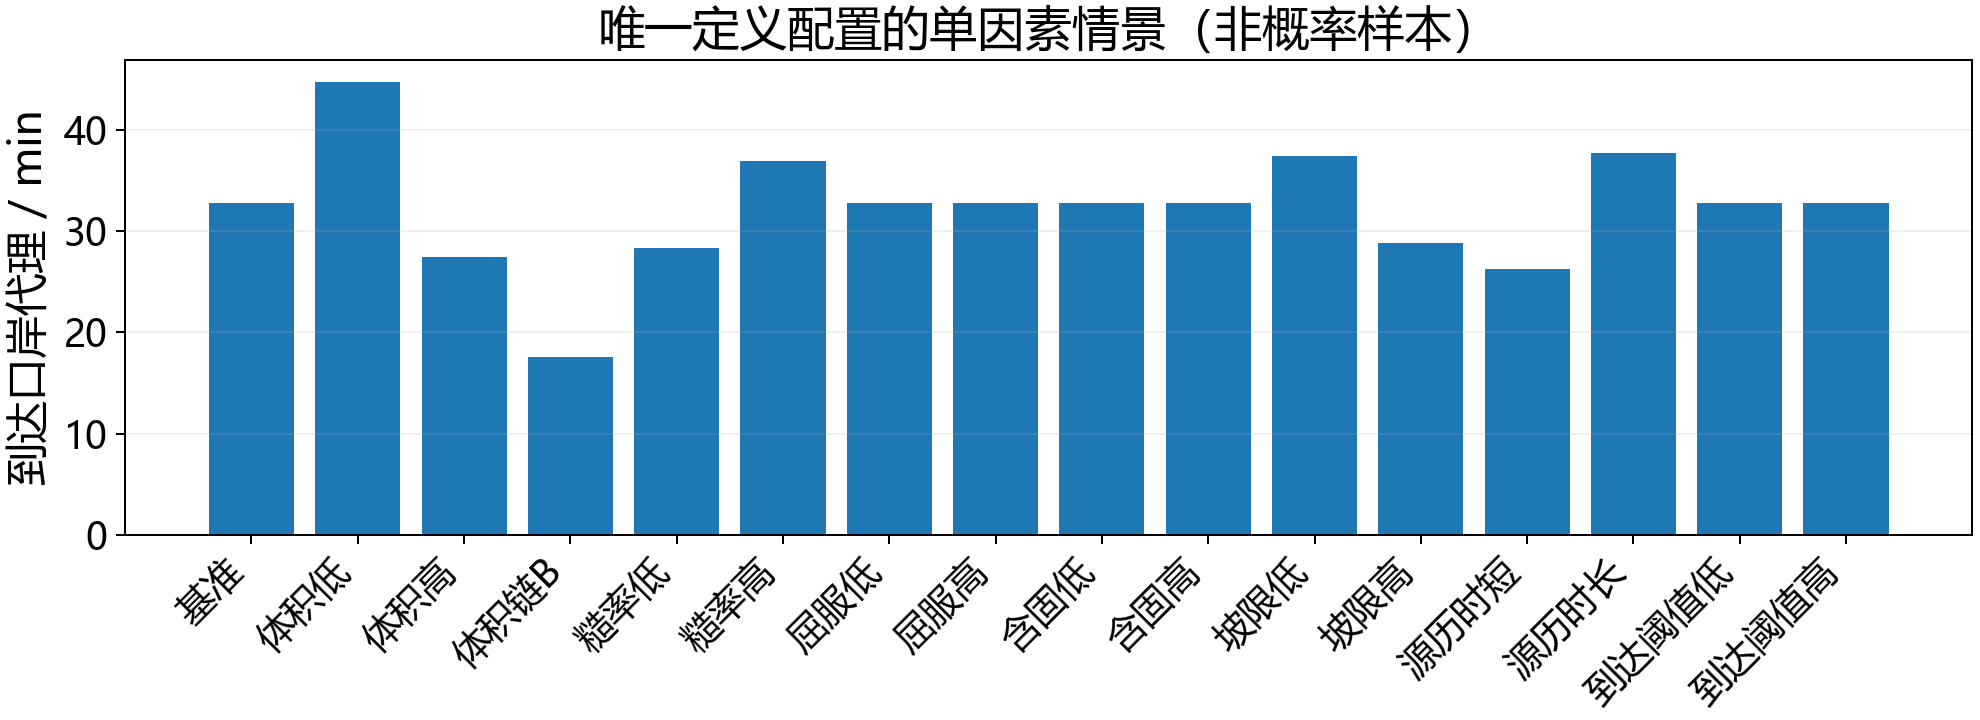
\includegraphics[width=0.96\textwidth]{04b_情景敏感性.png}
\caption{16个唯一D8配置的口岸到达时间（单因素情景，非概率样本）}
\label{fig:sensitivity}
\end{figure}

\subsection*{3.3 质量收支}
以实际注入体积为分母，基线最大相对质量残差为$2.075820191829099\times10^{-15}$，源项相对误差为0，全域最小深度非负，最大实际Courant数为0.188281359。图\ref{fig:mass}给出累计注入、域内、出域和损失体积的时间过程。数值闭合说明离散转移在机器精度内守恒，不说明地形时效、源区体积、屈服门槛或流变参数等于真实物理过程。

\begin{figure}[H]\centering
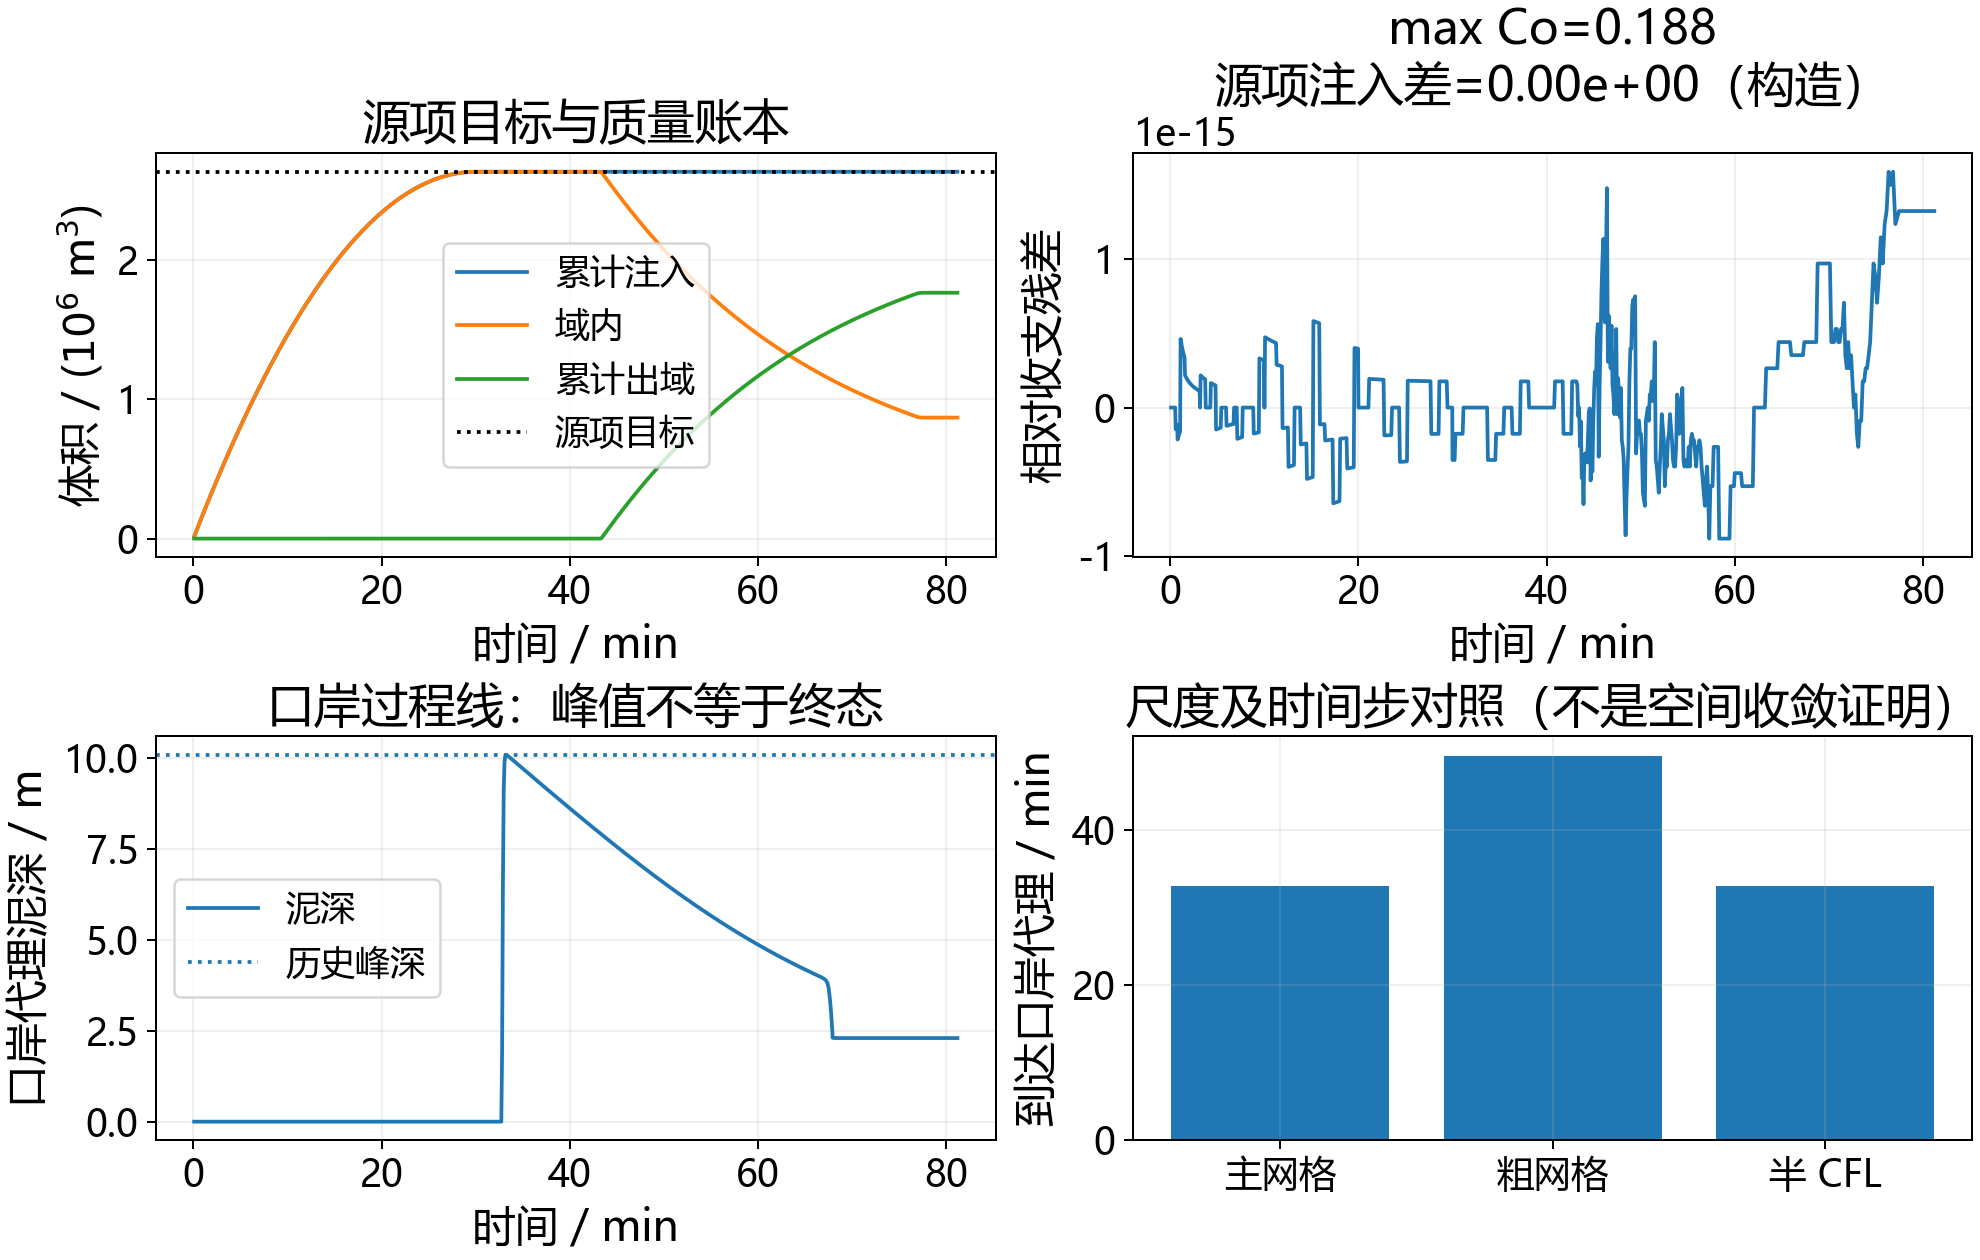
\includegraphics[width=0.96\textwidth]{04b_质量收支.png}
\caption{D8质量收支}
\label{fig:mass}
\end{figure}

\section*{四、结果摘要}
\begin{table}[H]\centering\small
\caption{D8基线结果与终止状态}\label{tab:summary}
\begin{tabular}{@{}l l@{}}
\toprule
指标&结果\\
\midrule
口岸代理首达时间&1965.996174 s，即32.7666029 min\\
16配置首达范围&17.5704376--44.7278067 min\\
口岸历史峰深&10.08530186 m\\
口岸终态深度&2.298002229 m\\
全域历史最大深&13.31272084 m\\
口岸峰值速度&6.601474228 m/s\\
质量相对残差&$2.075820191829099\times10^{-15}$\\
最大实际Courant数&0.188281359\\
终止状态&全部配置为域末端右删失\\
域末端里程&26045.4946703 m\\
\bottomrule
\end{tabular}
\end{table}

作为结构对照，一维基线在9.336769 km处自然能量停止，停止时间为1783.858032 s（29.73 min），未到达口岸；144个无节点配置中48个正速通过、96个首次停止。D8与一维的差异来自停止规则、有效断面宽度、缓坡驱动和路由结构，不是同一观测量的两次测量。

本文件中的图件均由\texttt{step04b\_sim2d.py}、\texttt{step04b\_map.py}、\texttt{step04c\_dynamics.py}及对应绘图脚本从同一结果数组生成；正文图10至图13与本文件图件同源。

\end{document}
